\documentclass{article}
%packages
\usepackage[english]{babel}
\usepackage[letterpaper,top=2cm,bottom=2cm,left=3cm,right=3cm,marginparwidth=1.75cm]{geometry}
\usepackage{amsmath}
\usepackage{graphicx}
\usepackage[colorlinks=true, allcolors=blue]{hyperref}
\usepackage{tikz}
\def\checkmark{\tikz\fill[scale=0.4](0,.35) -- (.25,0) -- (1,.7) -- (.25,.15) -- cycle;}

%Titel 
\title{Protokoll zu Meeting 28.02.2023}
\author{Lukas H�rnle}
%Begin of file
\begin{document}
    \maketitle

%Anwesenheitsliste 
    \section{Anwesenheitsliste}
    Anwesend waren folgende Personen:\newline
    \begin{table}[h!]
        \centering
        \begin{tabular}{l|r}
            Mitglied & Anwesend \\\hline
            Lukas H�rnle & \checkmark \\
            Marc G�kce & \checkmark \\
            Ralph Lausen & X \\
        \end{tabular}
        \caption{\label a Anwesenheitsliste}
    \end{table}


%Ziele des Treffens
    \section{Ziele}
    \begin{description}
        \item[Definition der Projektziele]
        Das Ziel und die wissenschaftliche Frage des Projektes sollen definiert werden.
        \item[Methoden zu Projektzielen]
        Methoden zur Umsetzung der Projektziele sollen festgelegt werden.
        Ein Ablaufplan hilft bei der Visualisierung
        \item[Zeitplan zu Meilensteinen]
        Es soll ein Zeitplan mit Zielen f�r einzelne Meilensteine des Projektes festgelegt werden.
    \end{description}

%Umgebung/Durchf�hrung des Treffens 
    \section{Umsetzung des Treffens}
    Das Meeting findet am 28.02.2023 von 15 bis 17 Uhr im Raum a264 an der DHBW Karlsruhe statt.
    Mithilfe der online verf�gbaren k�nstlichen Intelligenz ChatGPT\footnote{Siehe: \cite{ChatGPT}} werden Beispielthemen und Ans�tze im Bereich des zuvor definierten Tech Stacks unter Beachtung der Teamgr��e und bereits entschiedenen Themen generiert.
    Die generierten Themenans�tze werden nach Interesse und Komplexit�t bewertet.
    Ein Themenansatz mit angemessener Komplexit�t sowie bestehendem Interesse bei allen Beteiligten Entwicklern wird abgestimmt und ausgew�hlt.
    Eine kurze Recherche zu Trainingsdaten f�r eine kuenstliche Intelligenz bestaetigt die Themenwahl\footnote{Siehe: \cite{eecs.berkely}}.
    Eine beispielhafte Umsetzung wird oberfl�chlich mithilfe des Whiteboards erarbeitet.
    \subsection{Tafelanschrieb}
    \begin{figure}[h]
        \centering
        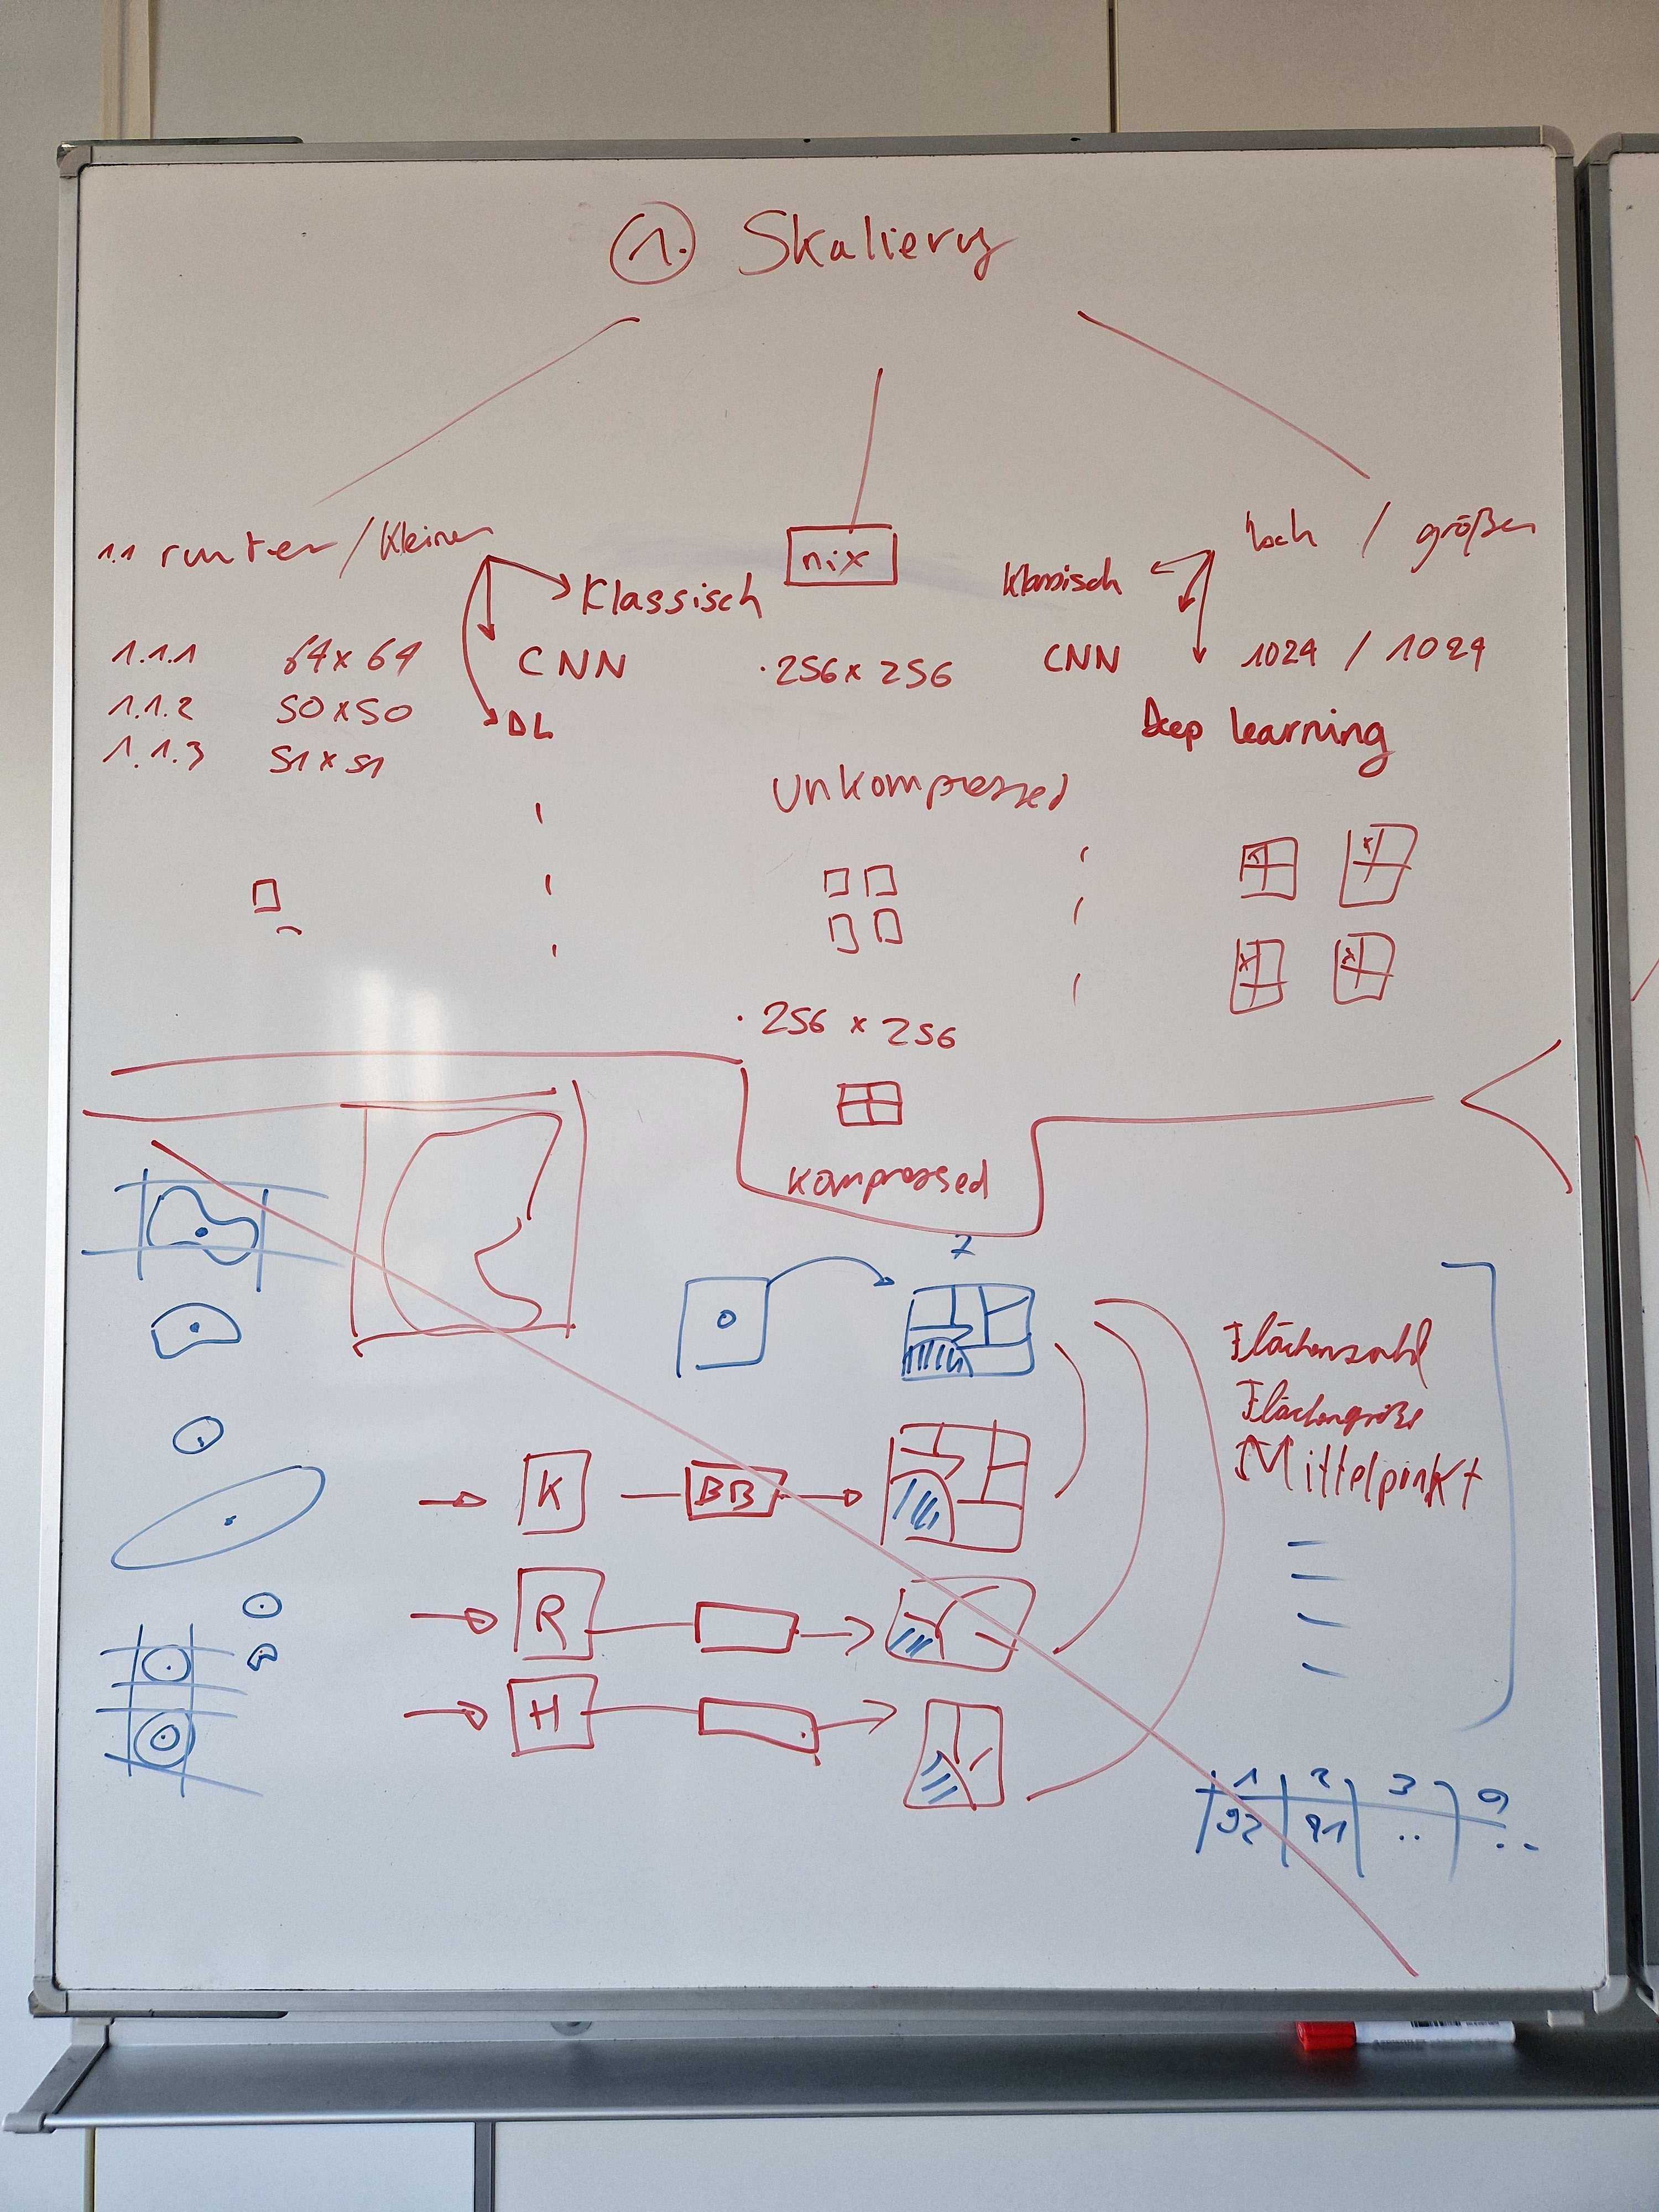
\includegraphics{Tafelanschrieb links}
        \caption{Tafelanschrieb zum Programmablauf (Linke Tafelh�lfte)}
        \label{fig:grafik_links}
    \end{figure}
    \begin{figure}[h]
        \centering
        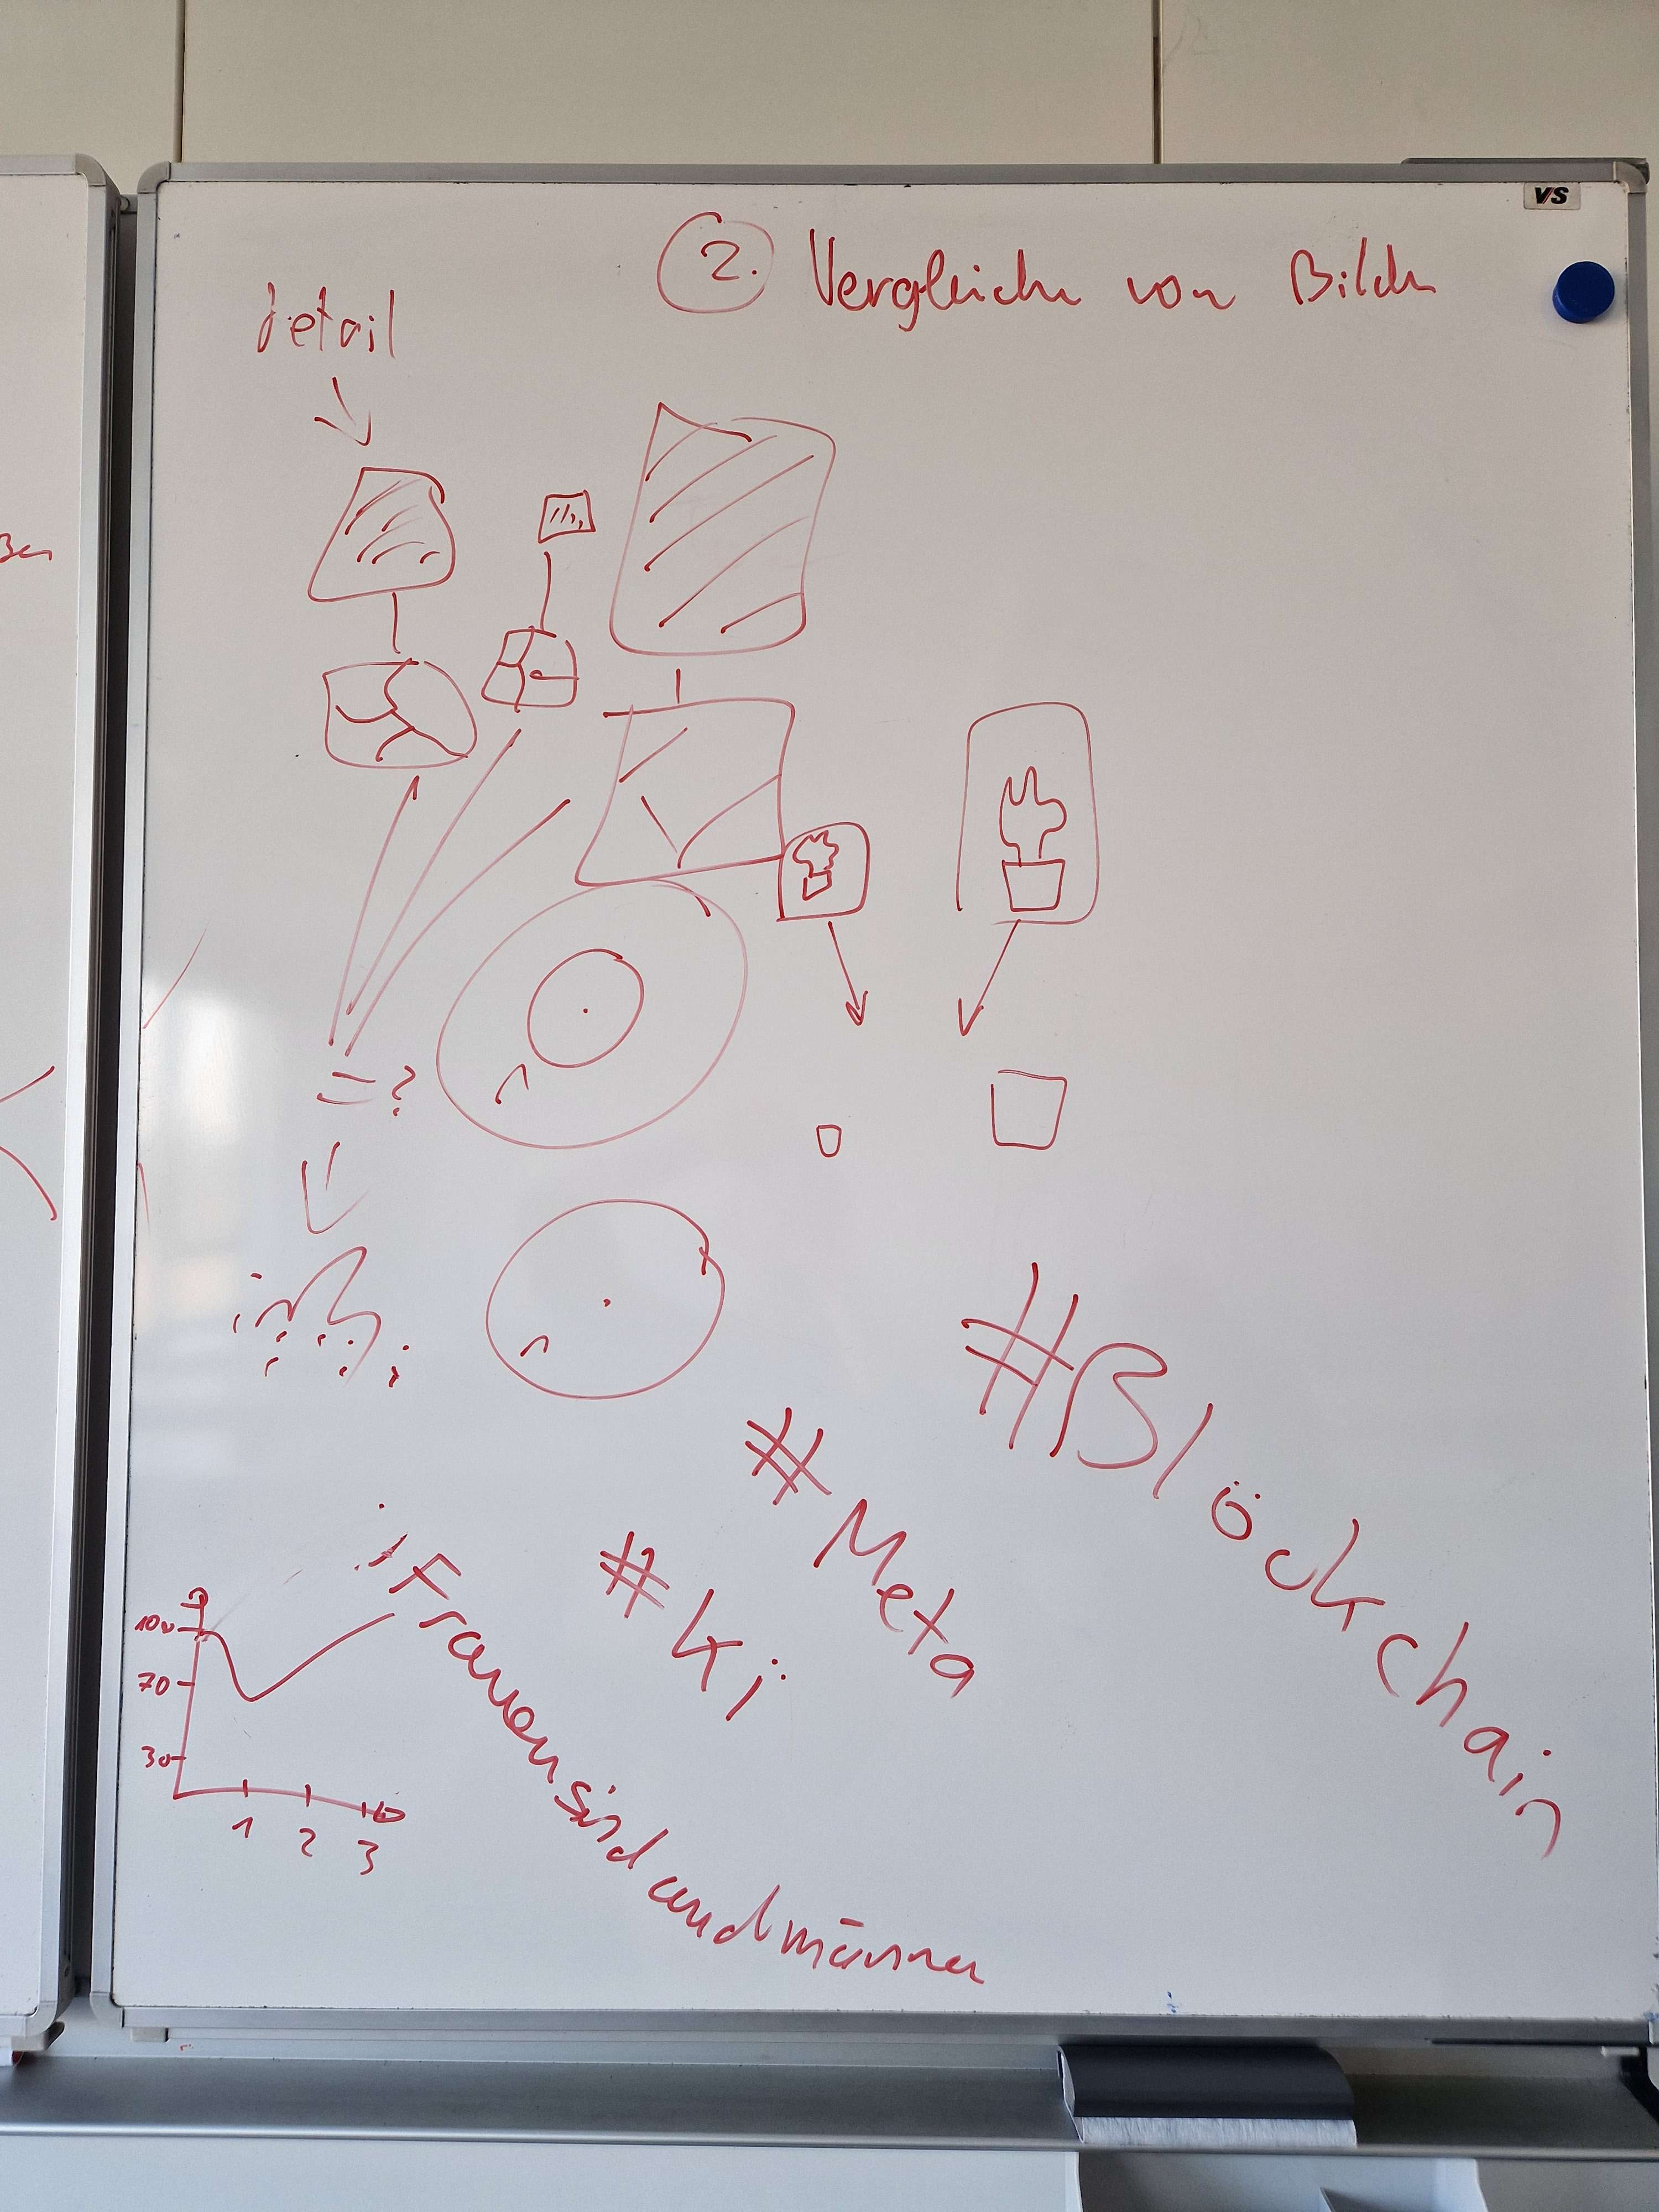
\includegraphics{Tafelanschrieb rechts}
        \caption{Tafelanschrieb zum Programmablauf (Rechte Tafelh�lfte)}
        \label{fig:grafik_rechts}
    \end{figure}
    Die Arbeit wird in Arbeitspakete und Meilensteine aufgeteilt.
    Diesen wird ein Zeitplan zugeordnet.
    \subsection{die vorl�ufige Gliederung und den Zeitplan bis zum Abgabetermin}
    28.02. Kickoff \newline
    4.3. klarstellen welche Daten wir nutzen \newline
    21.3. Skalierungsteil fertig entwickelt\newline
    01.04. Schreiben �ber Skalierung fertig\newline
    22.04. Segmentierung fertig. Entwicklungsstop\newline
    01.05. Schreiben fertig
    \subsection{Expos�}
    W�hrend des Termins werden alle wichtigen Inhalte in ein Expos� eingetragen.
    Dieses wird ansclie�end zur Dokumentation des Projektes vervollstaendigt
    Das Dokument wird der neuen Dokumentationssektion in Github hinzugef�gt \footnote{Siehe: \cite{GithubOrga}}
%Einbindung der Quellen
    \bibliographystyle{alpha}
    \bibliography{28022023}
%Dokumentenende
\end{document}